\chapter{Economics \small{\textsf{DRAFT}}}\label{chapter:economics}

So far, we have analyzed our protocols in the \emph{honest majority} setting,
assuming that most parties will follow our protocol. We provided assurances
such as safety and liveness to honest parties. But it's not clear why,
even though these assurances are provided, anyone should follow our honest
protocol, especially if they can achieve better benefits by deviating from
it. If there is money to be made by violating the protocol, it is likely that
a majority of participants will do so. Instead of assuming \emph{honesty},
it would make more sense to assume that participants are \emph{rational}.
A rational party does not necessarily follow the prescribed honest protocol.
Instead, he may deviate from the rules in order to make money.
The ideal scenario would be if the honest protocol we designed is also
\emph{incentive-compatible}\index{Incentive Compatibility}:
that there is no better strategy that
a party can follow which deviates from the honest strategy and makes them
more money (a Nash equilibrium).

\section{Rationality Models}

There are a few different models in which we can analyze our protocols.
In the \emph{cryptographic} model, the majority of parties are assumed
to be honest (and PPT), whereas the rest are allowed to be arbitrarily
adversarial (they can be any PPT algorithm). In the \emph{game theoretic}
model, \emph{all} parties are typically assumed to be rational, and
no computational restrictions are imposed upon them. However, the game
theoretic model does not typically account for adversaries who are willing
to deviate from the protocol even if they are about to lose money. Such
parties can be realistic in cases where, for example, a nation-state
wishes to invest resources simply to shut down a decentralized protocol.
But the cryptographic model \emph{does} capture such adversaries, as
long as most other participants are honest.

It would be nice to capture the best of both worlds. The most powerful
results would be achieved in a model where a \emph{majority} of parties
are assumed to be PPT rational, whereas a minority are assumed to be
\emph{arbitrarily PPT adversarial}. This is holy grail model and its
comparison to the other models is depicted in Figure~\ref{fig.rationality}.
Unfortunately, analyzing protocols in the rational majority setting
is very difficult with the current mathematical tooling available to us.
Analyzing the incentives of blockchain protocols is only possible for
very simple protocols, or for very simple models, and having an arbitrary
PPT adversary in the picture makes things even harder. While we would
like to have analyses in this model, it is rarely the case that we can.
There are many reasons for this, among others the complexity of the protocol,
the large number of parties, the broad range of available strategies,
the fact that the protocol is iterated over large periods of time,
and the fact that the practical instances of these protocols have externalities
such as payments that can be received outside of the protocol.

\begin{figure}[h]
  \centering
  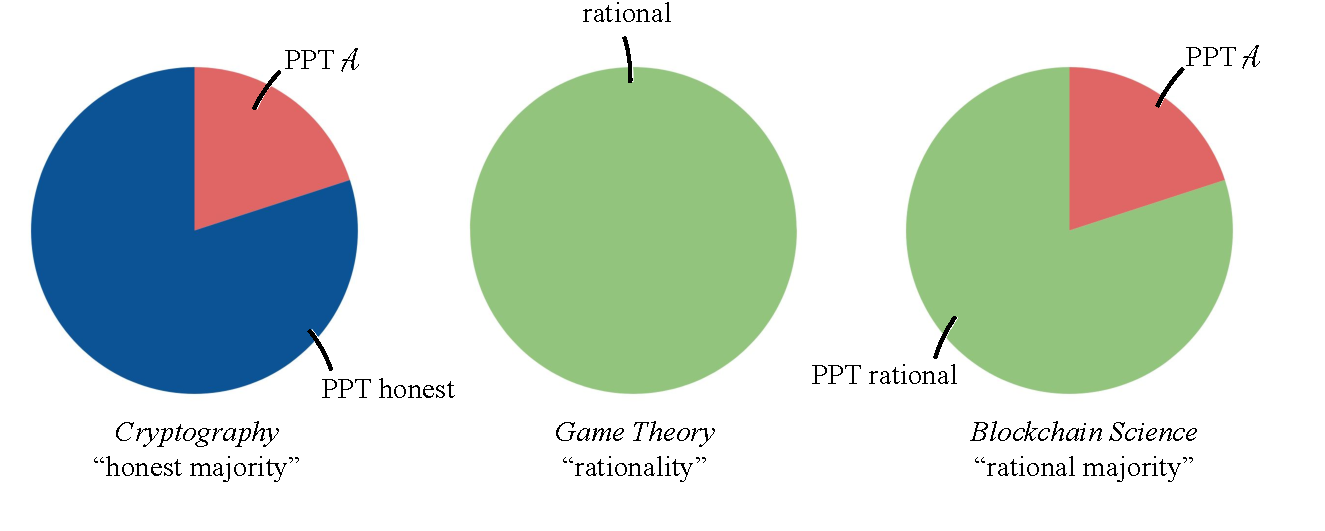
\includegraphics[width=\columnwidth,keepaspectratio]{figures/rational-model.pdf}
  \caption{The cryptographic, game theoretic, and blockchain science model.}
  \label{fig.rationality}
\end{figure}

Regardless of the limitations of our understanding and ability to prove
things precisely in the rational majority setting, it is still worthy
to think about the rationality of our design. While we might not be able
to prove that our honest protocol is incentive-compatible and survives against
arbitrary adversaries, we also want to make sure the honest protocol is
not costly to operate without providing appropriate incentives to honest
participants.

In the particular case of the proof-of-work protocol we have studied,
running the honest mining protocol is actually extremely costly. At the time of
writing, Bitcoin consumes more electricity than the whole country of Argentina,
which is an expensive endeavour. Therefore, miners need to be incentived to
secure the network, for example by having their electricity paid for.

We have already examined the mechanisms by which miners are paid when they
successfully mine a block in Chapter~\ref{chapter:chain}, where we mandated
that a block's coinbase transaction pays out a total amount $f_t$ which
consists of the \emph{block reward} $f_r$ and the \emph{block fees} $f_f$:

\[
    f_t = f_r + f_f
\]

Both of these terms are denominated in the system's native currency. We
will now study these two terms in more depth.

\section{The Block Reward}
The block reward part constitutes the \emph{macroeconomic policy} of the
system. This block reward plays a dual role for the system: Firstly, it
incentivizes miners to participate in the honest protocol. Secondly, it
is a natural mechanism for the decentralized creation of money. Whereas
the first purpose is necessary to make the protocol incentive-compatible,
the second part is a policy decision of the protocol. For example, it is
equally possible to have protocols in which new money creation is left up
to a central party, which can be the party to whom the newly issued money
is paid out to, and only a small proportion of the proceeds to go to the
miner. This would centralize money issuance, but still enable decentralized
public verifiability. Such decisions are a matter of policy.

The exact algorithm determining the value of $f_r$ is \emph{hard-coded}
into each full node and is part of the block validation algorithm. When
a block is validated, its coinbase is also validated, and this is where
the macroeconomic policy is checked for validity. It is typically not
possible to change these rules of the cryptocurrency, unless the community
of the currency all decide to move to a new policy and upgrade their software
together. Such decisions can be difficult and contentious.

% TODO: Write a small section on hard/soft forks and blockchain upgrades in
% this chapter.

There are a few alternatives that can be followed in the macroeconomic
policy of a cryptocurrency. The policy is defined as a function of the
block $f_r(B)$. One option is to make the reward \emph{constant}, which
means that the total supply will continue increasing at a constant rate.
Another option is to make the reward \emph{decreasing} over time until
it becomes $0$. In such a system, the function $f_r$ depends on the block
height. With such a policy, the total supply is increasing over time, but
converging to a particular value.

This is the policy that Bitcoin follows.
Bitcoin's macroeconomic policy is an interesting concrete example, because
many other cryptocurrencies follow a similar policy. The function $f_r$
for Bitcoin follows a staircase pattern, with long periods of constant
supply per block. The supply began at a rate of $50$ bitcoin per block
at genesis. Every four years in block time (which corresponds to
$210{,}000$ blocks because $\eta = 10$ minutes in Bitcoin), the reward
per block drops to a half (a process known as \emph{reward halving}).
The reward schedule for Bitcoin therefore
began at $50$ bitcoins per block during the years 2008-2012, dropped
to $25$ bitcoins per block during the next four years, and so on. At
some point in the future the block reward in Bitcoin will drop below
one Satoshi, at which point it will become $0$ and no new coins will
enter the supply. In about a century, Bitcoin will reach a total supply
of $21$ million bitcoin, and the reward will drop to $0$. This
macroeconomic policy is depicted in Figure~\ref{fig:reward_halving}
(in this graph by CoinDesk, \emph{subsidy} refers to the block
reward).

\begin{figure}[ht]
    \centering
    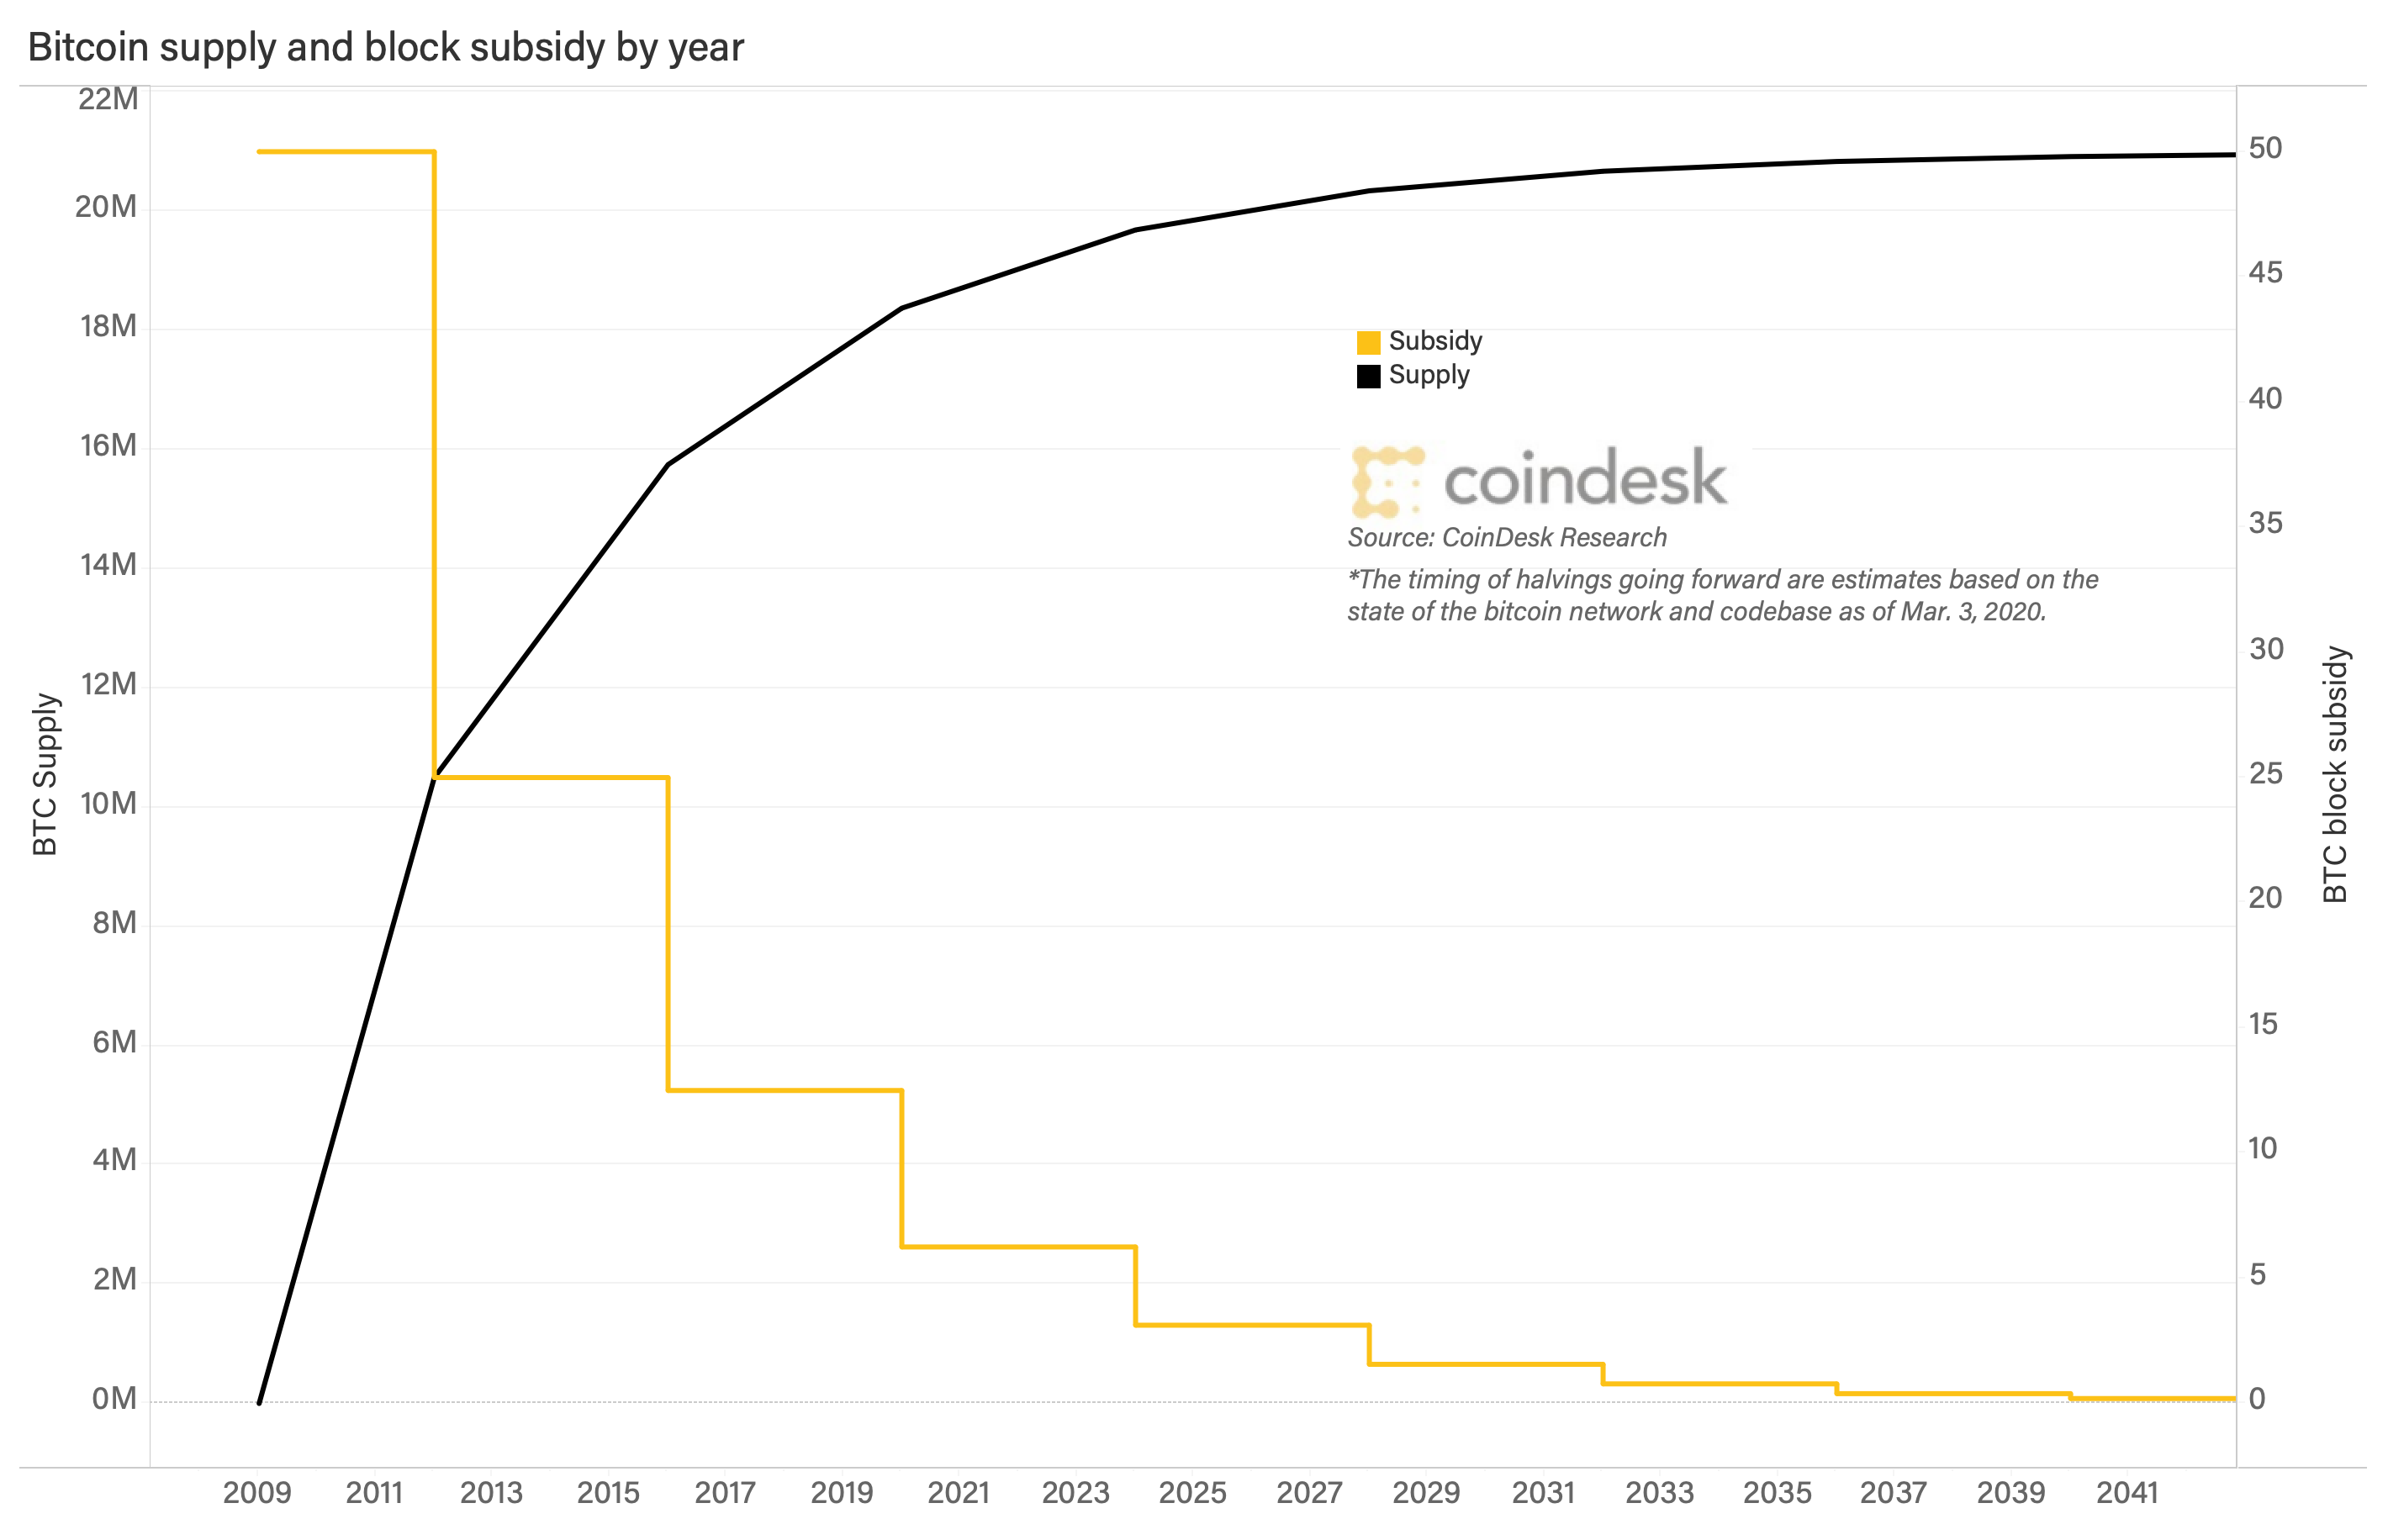
\includegraphics[scale = 0.2]{figures/reward_halving.png}
    \caption{Reward Halving for Bitcoin Supply\cite{halving}}
    \label{fig:reward_halving}
\end{figure}

One of the problems with such a policy is that the reward function
$f_r(h)$ is discontinuous with block height, and the finite difference
of the total supply function $\sum f_r$ changes abruptly at the points of
reward halving. This behavior can cause market shocks because the incentives
to the miners shift abruptly. Consider a miner who has invested in a large
business to mine blocks. The cost of electricity to mine is a certain
amount. At the moment of reward halving, the miner is still spending
the same amount per month in electricity, but only getting half of the
nominal rewards. Electricity is typically paid out in fiat (i.e., non-crypto)
currency such as USD. If the price of Bitcoin in USD remains the same, then
the miner will be forced to stop half of their operation overnight.
Alternatively, if the miner is to continue operating at the same rate,
the price of Bitcoin in USD needs to double overnight. Both of these
are undesirable situations.

To avoid such market shocks, other cryptocurrencies have adopted a more
nuanced macroeconomic policy. One such example is Monero which pioneered
the concept of \emph{smooth emission}. In such a system, the rewards
are reduced slightly in every block, following a pattern similar to
Bitcoin's macroeconomic policy, but adjusted to work in a more continuous
manner.

The reward and total supply functions for Bitcoin and Monero are
illustrated in Figure~\ref{fig.macroeconomics}. The actual
reward and supply over real (and not block) time can fluctuate less smoothly
than anticipated because of the stochastic nature of proof-of-work.
Note how Bitcoin's block reward forms a staircase, while Monero's
is a smooth curve. Due to a decision taken by the community, Monero's rewards
flatten out at the point indicated by the vertical red line.

% TODO: redo this figure
% https://www.reddit.com/r/Monero/comments/512kwh/useful_for_learning_about_monero_coin_emission/
\begin{figure}[h]
  \centering
  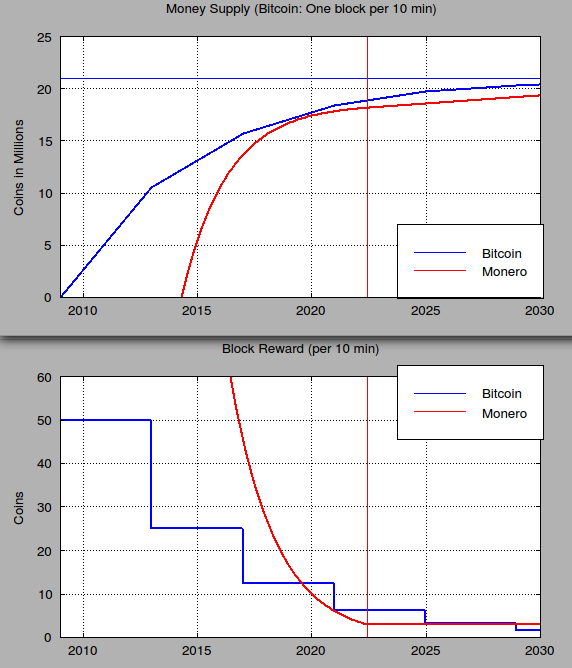
\includegraphics[width=0.8 \columnwidth,keepaspectratio]{figures/macroeconomics.png}
  \caption{The total supply (top) and block reward (bottom) for Bitcoin and Monero.}
  \label{fig.macroeconomics}
\end{figure}

Because the total supply stops growing at some point in time, Bitcoin
and Monero are \emph{deflationary cryptocurrencies}. Many orthodox
economists believe that deflationary cryptocurrencies are inappropriate
as currencies, because they encourage hoarding and not spending when
the emission period is over. This is one reason why other cryptocurrencies
have no limit on their total supply. Instead, they continue to inflate
the currency and are therefore known as \emph{inflationary cryptocurrencies}.
While it is important that the total supply of a cryptocurrency is limited
at every point in time to ensure scarcity, it is not necessary that there
is a global total bound across all of time. One such example cryptocurrency
is Dogecoin.

Overall, the decision of the macroeconomic policy of a system is up to
the economists and the community, and there is no exact science that can
define it in an objectively acceptable manner. Any emission algorithm
which is socially acceptable by the economic participants can be used.

The block reward is the main way miners are incentivized to mine.

\section{Miner Fee Optimizations}

While miners are incentivized to mine blocks by giving them a block reward,
they need to also be incentivized to include transactions in their blocks.
Otherwise, they will simply create \emph{empty blocks}\index{Empty Block},
blocks that contain only a coinbase transaction and don't confirm any
part of the mempool. This is solved by introducing transaction fees.

The other term of the total payout is the fees $f_f(B)$ of a block $B$.
Recall that the fees are calculated as the excess money that goes into
a transaction but does not go out. Given a transaction $\tx$ in the UTXO
model, the fees that this transaction is paying will be

\[
   \sum_{i \in \tx\textsf{.ins}} i.v - \sum_{o \in \tx\textsf{.outs}} o.v\,.
\]

The creator of a transaction can choose how many fees he wants to pay,
and these can be $0$ or larger.

Each block contains many transactions, each of which may pay out fees. All
these transaction fees make up the \emph{fee} part $f_f(B)$ of the block payout:

\[
  f_f(B) = \sum_{\substack{\tx \in B.\overline{x}\\\tx \textsf{ non-coinbase}}}
           \left(\sum_{i \in \tx\textsf{.ins}} i.v - \sum_{o \in \tx\textsf{.outs}} o.v\right)\,.
\]

Including an extra transaction has minimal cost to the miner and does not affect the mining
rate. If there was no limit in how big blocks can be, a rational miner would include all
transactions paying even minimal fees. But contrary to what we have described so far,
we will need to introduce a block size limit so that our assumptions can work out.

\subsection*{The Block Size Limit}

So far, we have not imposed any limits on how big blocks can be. We have also assumed
that blocks can traverse the network within $\Delta$ time, just like any other network message.
This should make you a bit suspicious by now. The larger a block is, the more time it
takes to send over the network. If we don't impose a bound on how large a block can get,
then $\Delta$ cannot be a fixed constant. There are some simple ideas to make blocks of
bounded size that don't work. One such example is to include just the transaction ids
within the block, and then allow the client to request each transaction as needed at
a later time. Another example is to just include the hash of the transaction sequence
$\overline{x}$, which already commits to the transactions, and not the transactions
themselves, again allowing the interested client to download the transactions in question.
We'll explore these strategies in more detail in Chapter~\ref{chapter:light} to optimize
our protocol, but for now let's observe why these don't fix the $\Delta$ problem:
The time $\Delta$ really captures the time that is needed for \emph{all} the data
to transmit over the network so that a block can be properly validated. If we separate
out transaction bodies from blocks, then a miner who observes a new block on the network
has to download all transactions in order to ensure block validity. Otherwise, the
miner cannot know if the block is valid or not and where to mine.

\glsxtrnewsymbol[description={block size limit}]{block size limit}{$\Bmax$}\glsadd{block size limit}
To ensure our assumption of a $\Delta$ delay holds, we will limit the size of a block
to $\Bmax$:

\[
    |B| \leq \Bmax
\]

This size limit must be denominated in actual \emph{bytes} (or bits) transmitted
over the network, not in the number of transactions per block. The reason is that the delay
$\Delta$ depends on the literal size of the object transmitted.

% TODO: Talk about how $\Delta$ can be decreased and the nodes who don't receive messages
% can be counted as part of the adversary, but this reduces the resilience. Maybe in a different
% chapter.

\subsection*{Miner Strategies}

Generally speaking, which transactions to include in a block is completely up to the miner,
as long as the block ends up being valid. The miner can choose to leave the block empty,
fill it to the brim, include transactions that are paying small fees, or include transactions
paying large fees. The miner can also include their own transactions at any position they
want within the block, and reorder the rest of the transactions in the block in any way
they like. Despite all of this freedom, some transaction inclusion \emph{strategies} are better than
others.

A rational miner is looking to optimize the fees that they can gain by including the highest
paying transactions that they can. When the miner is mining, they create a template block
in which the included transactions are $\overline{x}^*$. This $\overline{x}^*$ is computed
as follows. If the transactions in their mempool $\overline{x}$, plus
the new coinbase transaction, are enough to fit within $\Bmax$, then the miner has no reason
to exclude any transactions. He can simply include everything to maximize his profits.

On the other hand, if the mempool $\overline{x}$, plus the new coinbase transaction, exceed
the block size limit $\Bmax$ in size, then the miner must make a choice on which transactions
to include. He tries to maximize the profits by including the highest paying transactions.
In order to do that, each transaction is associated with a \emph{score}\index{Transaction Score}.
The score of a transaction is defined as the fees it is paying divided by the bytes it takes up:

\glsxtrnewsymbol[description={transaction score}]{transaction score}{$\score$}\glsadd{transaction score}
\[
    \score(\tx) = \frac{|\tx|}{\sum_{i \in \tx\textsf{.ins}} i.v - \sum_{o \in \tx\textsf{.outs}} o.v}
\]

The easiest way is then to order transactions by score, in descending order, and take
transactions until no more fit and $\Bmax$ would be exceeded. This strategy is also known
as the \emph{greedy strategy}\index{Greedy Strategy}. The reason why the ratio fee/byte
is used instead of just the fee is that, naturally, a bigger transaction takes up more space in
the block, and must therefore pay accordingly. This concept that block space costs a certain
amount per byte is also known as \emph{block space rent}\index{Block Space Rent}.

% TODO: write the greedy strategy in pseudocode

Unfortunately for the miner, things are not so simple. The first issue that arises is that
transactions can either be included \emph{as a whole} or \emph{not at all}. It is not possible
to cut a transaction in half and just include a portion of it into the block. This means that
the strategy to just include the top-score transactions will not perform optimally. One
such example is illustrated in Figure~\ref{fig.rational-miner-txs}. Here, the block is
illustrated as the outer blue box, with its size indicating the block size limit $\Bmax$.
Transactions in the mempool (breaking away from our usual circle
notation) are displayed as smaller boxes containing numbers. The numbers within the transactions
indicate their score, and the size of a box indicates the transaction's size in bytes.
The transactions have been ordered by the greedy strategy from left to right in
descending order according to their scores. The green transactions are included in
the block, as they are the transactions with the top scores. The red transactions
are not included in the block, as they have lower scores. The transaction with
a score of $4$ barely doesn't fit in the block. However, the greedy strategy misses
the fact that the two smaller transactions with a score of $3$ can both still fit in
the block. A more clever solution would include these also. If it were possible to cut the
transaction with the score of $4$ and partially include it, then this solution would
have been optimal, but we are forced to exclude it altogether, so the transactions
with a score of $3$ are our next best option.

\begin{figure}[h]
  \centering
  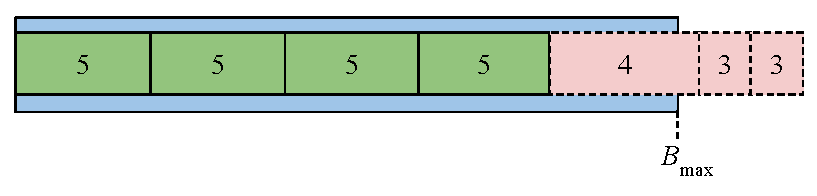
\includegraphics[width=0.8 \columnwidth,keepaspectratio]{figures/rational-miner-txs.pdf}
  \caption{The greedy strategy is not always optimal.}
  \label{fig.rational-miner-txs}
\end{figure}

This problem is known as the $0/1$ Knapsack problem and is known to be an NP-hard problem.
Its best known solution is only pseudopolynomial (which means it takes exponential time to
execute). Therefore, the problem of optimizing
which transactions to include is, generally, difficult, and only heuristics can be employed
to solve it. These heuristics sometimes necessarily yield suboptimal solutions.

Even this simple rendition of the problem is NP-hard, but in fact the problem is harder still.
The transactions that can be included must also respect the topological order induced by
the transaction graph. We cannot include a transaction $\tx_1$ before the transaction $\tx_2$
it is spending from. Therefore, the problem is similar to a $0/1$ Knapsack, except that
topological relations must also be preserved.

Lastly, there is one more complication. The simplistic honest miner maintains a mempool
that outright rejects double spends. This is fine for a miner who is not interested in
maximizing his profits. However, a rational miner wants to keep track of double spends.
If two conflicting transactions $\tx$ and $\tx'$ are available, the miner wishes to
choose the one with the highest paying fee. Even if a double spending transaction does
not pay large fees, it may still worth be caching for later inspection, because it may
be the input to a next transaction that \emph{does} pay large fees. Therefore, a rational
miner will also cache transactions outside of his mempool and hold onto them in case
they are later helpful in optimizing his profits.

In complex blockchains, such as Ethereum, the order of transactions in a block may give rise
to more nuanced profits than just those obtained from fees, and so even more advanced techniques
are needed. The strategies employed by modern rational miners to optimize profits are extremely
complicated and have given rise to a whole industry on their own. In the modern world,
\emph{computing} the near-optimal $\overline{x}^*$ and actually \emph{mining} a block
are two separate tasks. The computation of $\overline{x}^*$ is a task performed by
\emph{searchers} and \emph{builders}, whereas the mining is performed by \emph{miners}.
These are different, somewhat mutually trusted, parties running different software and
communicating with one another to optimize rational block production and share these
profits, which can range to tens of millions of dollars per month.

\section{Wallet Fee Optimization}

While the miner is trying to \emph{maximize} their fees, the \emph{wallet} of the user
who is spending money is trying to \emph{minimize} their fees. What is observed on-chain
is the economic equilibrium between the two.

Refer back to Figure~\ref{fig.wallet-fullnode-architecture} to recall that the wallet
is the piece of software that sits between the human user and the full node. The job of
the wallet is to take requests from the human user to make payments, and to issue the relevant
transactions to make these payments. The human user places such a request by choosing a particular
recipient and value to transfer. It is up to the wallet to decide how to build the transaction.

First, the human user places a request to the wallet to make a payment of amount $v$ to some
recipient $pk$. a transaction, the wallet obtains the UTXO set from the full node it is
associated with and must choose

% \section{Some Bitcoin Statistics}
% We can take a look at the blockchain statistics for Bitcoin on the website:\\
% \href{https://www.blockchain.com/charts/hash-rate}{https://www.blockchain.com/charts/hash-rate}.
% Today, the hash rate of the bitcoin network is $210.48$m TH/s, measured in terahertz per second, as shown in Figure ~\ref{fig:hash_rate}. This can be denoted as:
% \begin{align*}
%     q\cdot (n-t) \approx 2^{67} \texttt{ Hz}.
% \end{align*}
%
%
% \begin{figure}[ht]
%     \centering
%     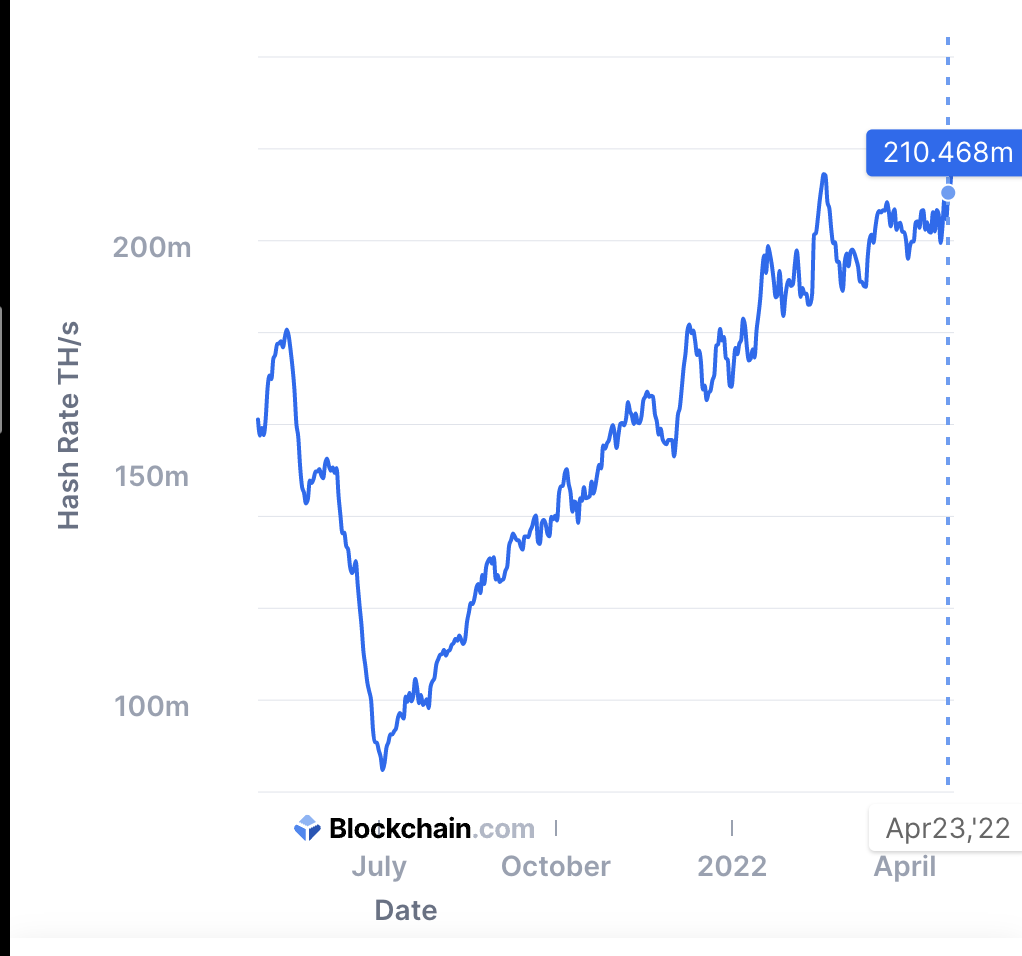
\includegraphics[scale = 0.6]{figures/hash_rate.png}
%     \caption{Hash Rate of Bitcoin from April 2021 to April 2022\cite{hash-rate}}
%     \label{fig:hash_rate}
% \end{figure}
%
% We can estimate the value of $q$ (the hash power of 1 party) on a real computer. On a laptop, $q \approx 100 \texttt{MHz}$. On a GPU, we can raise this to $q \approx 20 \texttt{ GHz}$. Today, we also use specialized mining power, with the best machines (ASICs) achieving $q \approx 200 \texttt{ THz}$. To see the hash power of the ASIC machine, you can refer to this website: \href{www.asicminervalue.com}{www.asicmine
% rvalue.com}
%
% We can also use the website to examine the number of transactions that are confirmed in any time frame. Here are some other observations:
% \begin{itemize}
%     \item The number of transaction spikes in the weekdays and toughs on the weekends
%     \item The number of UTXOs grew significantly in the past year
%     \item The mempool size is more erratic
% \end{itemize}
% Overall, observe that many network activity values depend on human factors.

\section{Mining}

\subsection{Including a transaction}
Since miners prefer to mine more profitable transactions (i.e. those with higher fees), the chosen transaction fee would determine the confirmation time for a transaction. If a wallet wants their transaction to be confirmed faster, they would set a higher fee to incentivize miners to include the transaction into their blocks. If the wallet pays a lower fee, the transaction may take longer to be included, or never be included.

\section{Variable Mining Difficulty}
The Marabu protocol has a constant difficulty parameter, and thus a constant target $T$. However, this creates a problem since the hash power of the network is constantly changing. Therefore, when the hash power increases, the rate of block production could be less than $\Delta$. To keep a desired block production rate, we want to scale the difficulty appropriately as the hash power of the network increases.

\subsection{Definitions}

\begin{definition}
    Let $f$ be the probability of getting an honest block in one unit of time. Then,
\begin{align*}
    f &\approx p \cdot q \cdot (n-t) \\
    f &= 1- (1-p)^{q(n-t)}
\end{align*}
where $(1-p)^{q(n-t)}$ is the probability that every honest party failed.
\end{definition}
In Bitcoin, where 1 block is produced approximately every 10 minutes, we have $f \approx 1/600$ seconds. For small $p$, we have
\begin{align*}
    (1-p)^{q(n-t)} \approx 1 - qp(n-t)
\end{align*}

\begin{definition}
Let $\eta = \frac{1}{f}$ be the expected block production duration.
\end{definition}
We split the chain into sections $m$ blocks long.
\begin{definition}
Let an \textit{epoch} be a section that is $m$ blocks long, where $m$ is a constant.
\end{definition}
Given the target for epoch $j-1$, denoted $T_{j-1}$, we wish to find the target for the next epoch $T_j$. The desired epoch duration is $m\cdot \eta$, the number of blocks times the expected production rate, but the actual duration is $t_2-t_1$ where $t_1$ and $t_2$ gives the mining times of the first and last blocks of the epoch $j-1$, respectively. Then we recalculate the target via

\begin{align*}
    T_j = T_{j-1}\frac{t_2 - t_1}{m\eta}
\end{align*}

We reach the following conclusion:
\begin{quote}
If actual time $<$ desired $\longrightarrow$ target decreased, difficulty increased.\\
If actual time $>$ desired $\longrightarrow$ target increased, difficulty decreased
\end{quote}

\section{Mining Pools}
The probability of an individual miner successfully mining a block (and earning \$200k for the reward) is low. This reward has a high expectation, but it also has high variance. However, the miners want a consistent return, with the same expectation but a lower variance. To do this, miners combine together to form a \textit{pool}.

\begin{definition}
A \textit{pool} is a collaboration of miners. If any one miner succeeds, then they share the profit with other miners.
\end{definition}

\subsection{How Pools Work}
The pool operator, a trusted party, generates a key pair ($pk, sk$) and shares the public key $pk$ with all miners. The participants mine the block, in which the coinbase transaction goes to the public key $pk$ of the pool operator. Then, the operator distributes profits to the miners.

Now the pool operator must verify that the miners are actually mining. They could achieve this by setting up a light PoW verification.
\begin{definition}
The \textit{light PoW} equation provides a target that is significantly easier, called a \textit{light block share}:
\begin{align*}
H(B) &\leq 2^\xi T
\end{align*}
where $\xi$ denotes a constant that scales the target.
\end{definition}
The participants would send the light PoW block to the operator once they have mined a block. The operator validates that:
\begin{enumerate}
    \item The light block share satisfied the light PoW equation
    \item The coinbase pays the operator\end{enumerate}

Finally, after the block is mined, the operator distributes profits in proportion to the shares reported. An adversarial miner can only get payed if they submit the valid light block share. Additionally, the miner cannot change a valid block's public key to their own address because this will change the hash. Finally, an adversary would want to share a found block because they would get rewarded as part of the pool.

\section{Wallets}

\subsection{Mining and Wallets}
While miners wish to maximize fees to increase their rewards, wallets wish to minimize fees to decrease the price of transactions. The fee-per-byte is fixed by the user, so one way to lower the transaction fee is to minimize the size in bytes of the transaction. In case a user miscalculates the fee-per-byte and gives a value that is too low, an honest user can submit the same transaction but with a higher fee. This is an ``honest" double spend called a \textit{replace by fee}, as shown in Figure \ref{fig:replace_by_fee}. The higher-fee transaction replaces the older one in the mempool.

\begin{figure}[ht]
    \centering
    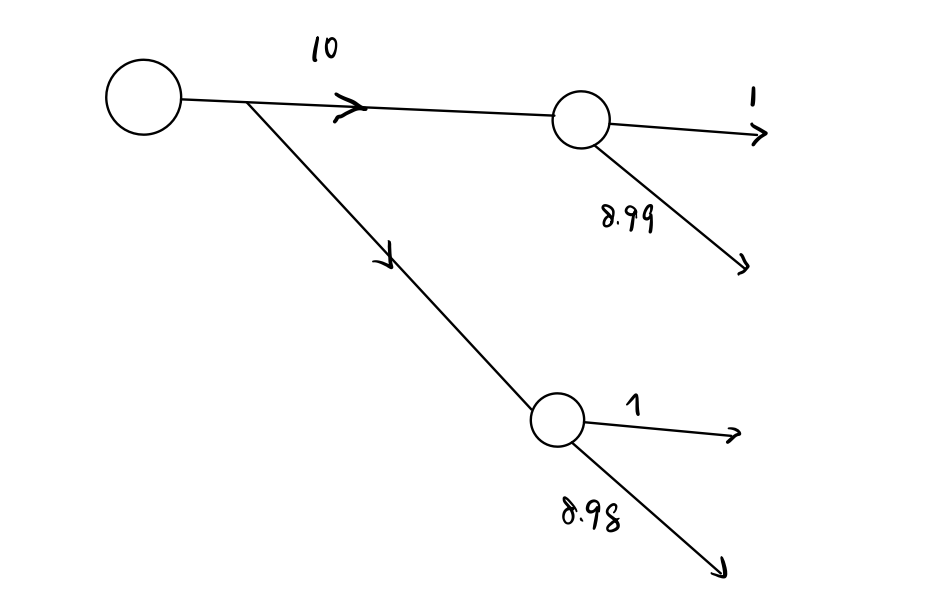
\includegraphics[scale = 0.5]{figures/replace_by_fee.png}
    \caption{An example of a honest, rational party not being able to send a transaction and creating another replace by fee transaction}
    \label{fig:replace_by_fee}
\end{figure}


\subsubsection{Types of Wallets}
Wallets can be ``hot" or ``cold". Hot wallets are online, so they are easily available to use but less secure. Cold wallets are stored offline, such as in a hardware wallet or written down on a piece of paper. The hardware wallet could be plugged into a computer. The computer would store the transaction information, while the wallet generates the public keys, secret keys, and the signature without the secret keys leaving the device. They are more secure but tend to be harder to operate.


\begin{figure}[ht]
    \centering
    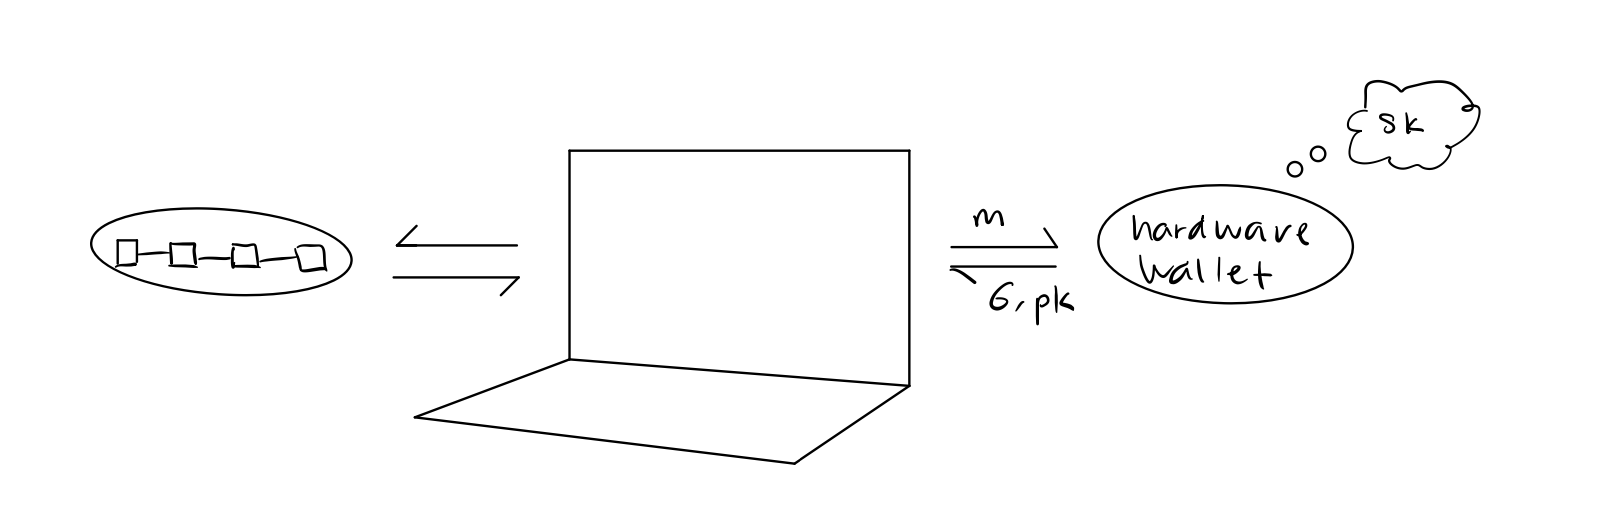
\includegraphics[scale = 0.5]{figures/hardware.png}
    \caption{Illustration of the interactions between the hardware wallet and the computer}
    \label{fig:hardware}
\end{figure}

\begin{figure}[ht]
    \centering
    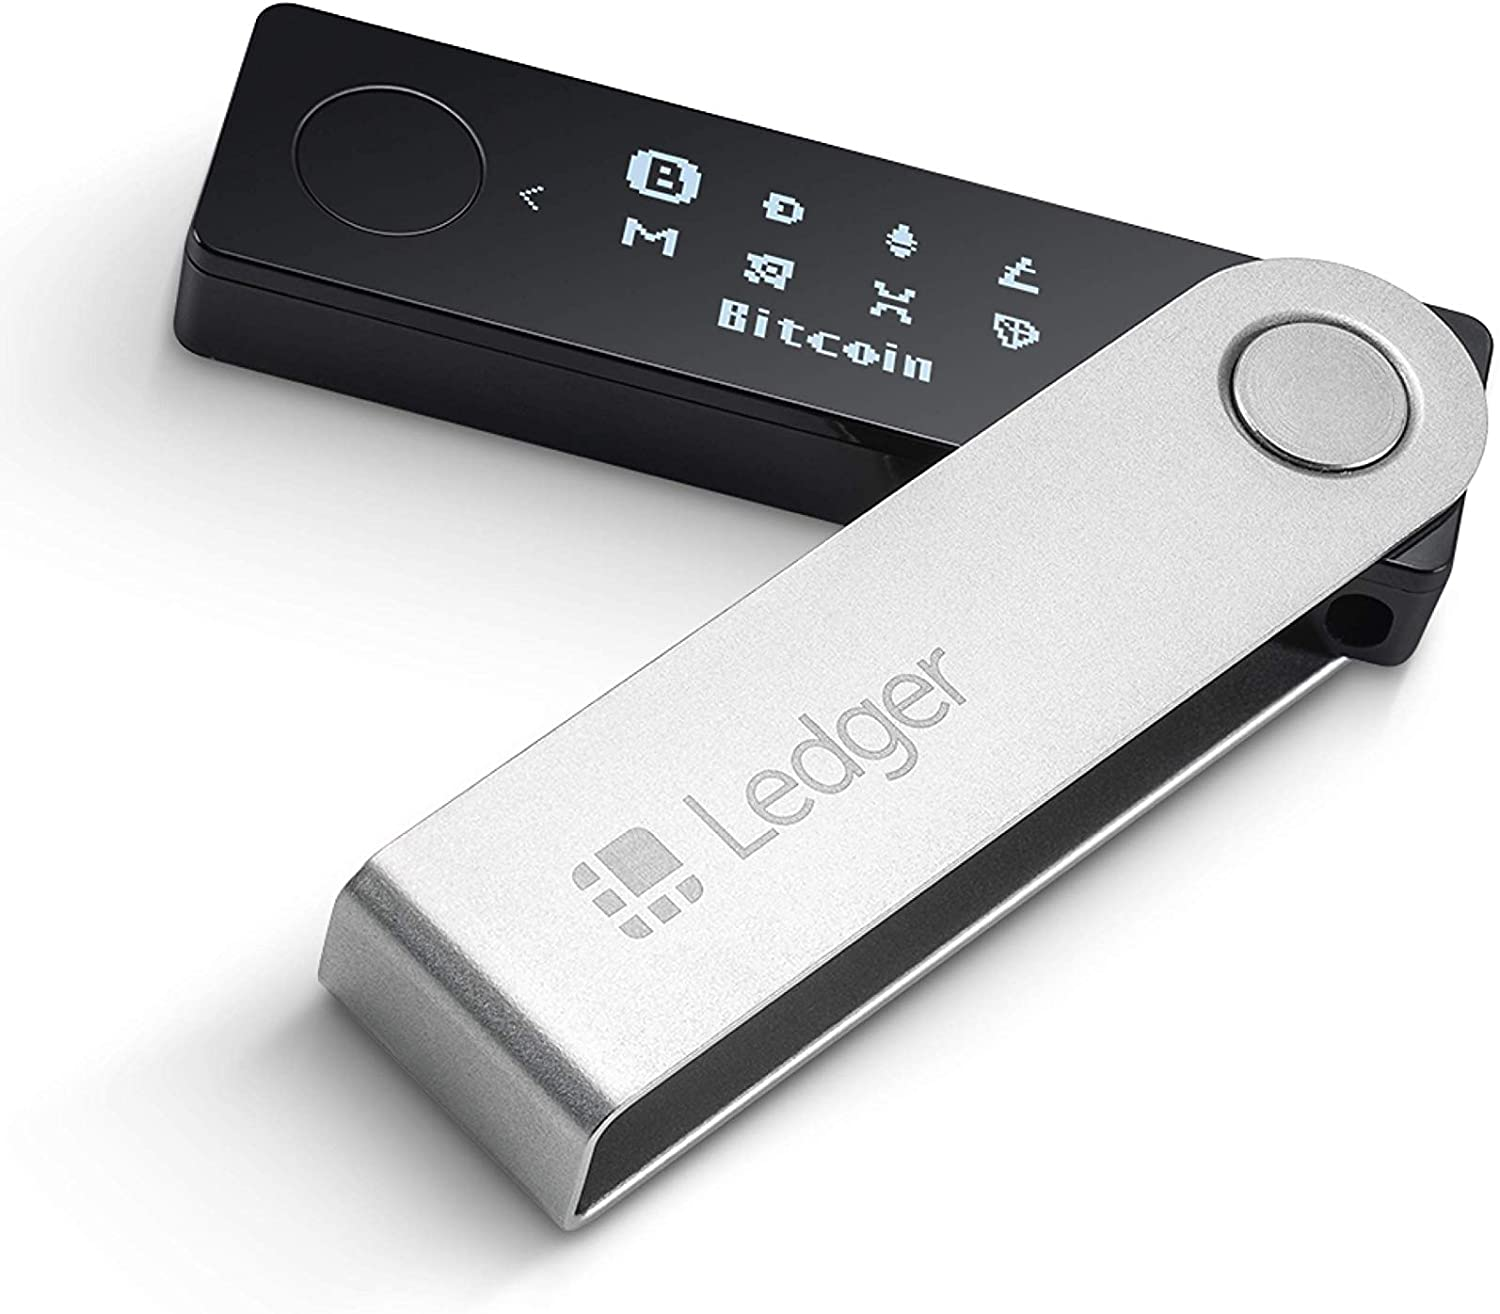
\includegraphics[scale = 0.1]{figures/hardware_wallet.jpg}
    \caption{An Example of a Hardware Wallet\cite{hard}}
    \label{fig:hardware_wallet}
\end{figure}


\subsection{HD Wallets}
For a wallet, we want to generate public and secret key pairs (sk, pk) $\longleftarrow$ $\mathsf{Gen}(1^\kappa)$.

To do this, one approach is to start with a seed that is randomly generated (such as a series of words), then hash the seed with a counter. Note that we cannot use human-generated random words, such as ``I love my dog", because it could be easily stolen.

One commonly used approach is the following. Given a randomly generated \textit{seed}, we can concatenate it with a counter and hash the concatenation to achieve a new secret key. Then, from the secret key, we can generate a public key.
\begin{align*}
H(\text{ctr}\|\text{seed})&\longrightarrow \text{new sk} \\
H(1\|\text{seed}) &\longrightarrow \text{new sk}_0  \\
H(2\|\text{seed}) &\longrightarrow \text{new sk}_1 \\
&\cdots
\end{align*}

\section*{Problems}
TBD

\section*{Further Reading}
While it is folklore belief that a cryptocurrency can remain incentive-compatible
when payouts consists only of block rewards and no fees, this belief is actually
false. This was studied in the paper
\emph{On the Instability of Bitcoin Without the Block Reward}~\cite{instability}.

The field of optimizing miner strategies was pioneered by two works,
\emph{Clockwork Finance}~\cite{clockwork} and \emph{FlashBoys 2.0}~\cite{flashboys}.
These gave rise to the concept of \emph{MEV}, or Miner Extractable Value, and
gave rise to a whole industry of \emph{searchers}, \emph{builders}, and \emph{proposers},
allocating different roles to the different portions pertaining to this optimization
problem. The most popular platform in the field currently concerning itself with
such optimizations is \emph{FlashBots}.
